\chapter{线性代数}
\label{ch:linear_algebra}

线性代数是广泛使用在整个科学和工程中的一个数学分支。然而,由于线性代数是一种连续
的形式而不是离散数学,许多计算机科学家对它少有经验。很好地理解线性代数,对理解和
使用许多\gls*{ml}算法来工作,是必不可少的,对\gls*{dl}尤其如此。因此,我们在介
绍\gls*{dl}之前先专注于对关键的线性代数必备知识做些陈述。

如果你已经熟悉了线性代数,尽管跳过这一章。如果你对这些概念有了一些先期的经验,但
是需要一个详细的参考来复习关键的公式,我们推荐 \emph{The Matrix Cookbook}
\citep{matrix-cookbook}。如果你完全没有接触过线性代数,这一章会教你足够的知识来阅
读本书,但是我们强烈建议你也去咨询其它专门教授线性代数的材料,例
如\citep{shilov1977linear}。本章会完全略过很多重要的线性代数的主题,它们对理
解\gls*{dl}不是必须的。

\section{标量、向量、矩阵和张量}
\label{sec:scalars_vectors_matrices_and_tensors}

线性代数的研究涉及到几种数学对象的类型:

\begin{itemize}
\item \emph{\gls{scalars}}:一个标量仅仅是一个单独的数字,相反,大多数其它线性代
  数的研究对象通常是多个数组。我们用斜体来写标量。我们通常用小写命名标量。当我们
  介绍它们时,我们指定它们是什么样的数字。例如:当定义一个实数值的标量时,我们可
  能说``设 $s \in \mathbb{R}$ 为直线的斜率'',或者,当定义一个自然数标量
  时,``设 $n \in \mathbb{N}$ 为单元的个数''。
\item \emph{\gls{vecs}}:一个\gls*{vec}是一个数组。这些数字按照顺序排列。我们可以
  通过这一顺序中的索引来确定每一个单独的数字。通常我们以小写的粗体字体
  给\gls*{vec}命名,例如 $\pmb{x}$。\gls*{vec}的元素以伴有下标的斜体字体表
  示。$\pmb{x}$ 的第一个元素是 $x_1$,第二个是 $x_2$,依此类推。我们还要说
  明\gls*{vec}中存储的是什么类型的数字。如果每个元素是 $\mathbb{R}$ 中的数,
  而\gls*{vec}有 $n$ 个元素,那么\gls*{vec}位于以 $\mathbb{R}$ 的 $n$ 次笛卡尔积
  的所形成的集合内,表示为 $\mathbb{R}^n$。当我们需要显式地表示一个\gls*{vec}中的
  元素,我们把它们写成方括号围起来的一列:
  \begin{equation}
    x = \begin{bmatrix}x_1\\ x_2\\ \vdots\\ x_n\end{bmatrix}
    \label{eq:vec_example}
  \end{equation}
  我们可以把\gls*{vec}看做表示空间的点,每个元素提供沿着不同坐标轴的坐标。\\
  有时候我们需要索引一个向量中的一个元素集合。在这种情况下,我们定义一个包含索引
  的集合,并把这个集合写成一个下标。例如,为了获得 $x_1$,$x_3$ 和 $x_6$,我们定
  义集合 $S = {1, 3, 6}$,写为 $\pmb{x}_S$。我们使用 $-$ 标记表示一个集合的补充。
  例如 $\pmb{x}_{-1}$ 是包含 $\pmb{x}$ 中除了 $x_1$ 的所有元素
  的\gls*{vec},而 $\pmb{x}_{-S}$ 是包含 $\pmb{x}$ 中除了 $x_1$,$x_2$ 和 $x_6$
  之外的所有元素的向量。
\item \emph{\gls{matrices}}:一个矩阵是一个数字的二维数组,所以每个元素由两个索引
  确定,而不是一个。我们通常用大写的粗体字体表示矩阵,例如 $\pmb{A}$。如果一个实
  数值的矩阵 $\pmb{A}$ 高度为 $m$,宽度为
  $n$,那么我们说$\pmb{A} \in \mathbb{R}^{m \times n}$。我们通常使用斜体~——~但不
  是粗体字体~——~表示一个矩阵的元素,索引用逗号分开列出。例
  如,$A_{1,1}$ 是 $\pmb{A}$ 左上角的元素,而 $A_{m,n}$ 是右下角的元素。我们可以
  为横向坐标写一个 ``:'' 来表示所有竖向坐标 $i$ 的数字。例如,$\pmb{A}_{i,:}$ 表
  示竖向坐标 $i$ 的横跨 $\pmb{A}$ 的部分。即 $\pmb{A}$ 的第 $i$ 行。同样
  的,$\pmb{A}_{:,i}$ 是 $\pmb{A}$ 的第 $i$ 列。当我们需要显式地表示一个矩阵的元
  素,我们把它们写成一个用方括号围起来的数组:
  \begin{equation}
    \begin{bmatrix}A_{1,1} & A_{1,2} \\ A_{2,1} & A_{2,2}\end{bmatrix}
    \label{eq:matrix_example}
  \end{equation}
  有时候我们可能需要索引矩阵值的表达式,它不仅仅是一个单个的字母。在这种情况下,
  我们在表达式后使用下标,但不转换为小写。例如,$f(\pmb{A})_{i,j}$ 给出了应用函
  数 $f$ 到 $\pmb{A}$ 上后计算得到的 $(i,j)$ 位置的元素。。
\item \emph{\gls{tensors}}:在有些情况下我们会需要一个多于两个坐标的数组。在一般
  情况下,排列在一个规则的网格~——~具有可变数量的坐标轴~——~上的数组,被称为一
  个\emph{\gls{tensor}}。我们用这样的字体表示一个名为 ``A'' 的张
  量:$\pmb{\mathsf{A}}$。我们把表示 $\pmb{\mathsf{A}}$ 在 $(i,j,k)$ 坐标的元素写
  为 $\mathsfit{A}_{i,j,k}$。
\end{itemize}

矩阵的一个重要的操作是\emph{\gls{transpose}}。一个矩阵的\gls*{transpose}是将矩阵
沿着一个对角线~——~称为\emph{\gls{main-diag}},从左上角指向右下角~——~做镜像。参见
图~\ref{fig:transpose_of_matrix} 中对这个操作的图形化描述。我们把一个矩
阵 $\pmb{A}$ 的转置表示为 $\pmb{A}^{\top}$,以这样定义
\begin{equation}
  (\pmb{A}^{\top})_{i,j} = A_{j,i}
  \label{eq:transpose_of_matrix}
\end{equation}

\begin{figure}[h]
  \centering
  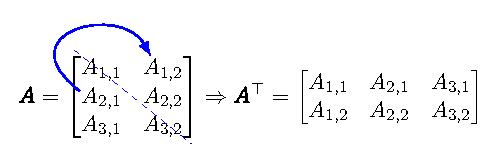
\includegraphics{transpose_of_matrix}
  \caption{矩阵的转置可以被看做沿着\gls*{main-diag}的镜
    像\label{fig:transpose_of_matrix}}
\end{figure}

\gls*{vecs}可以被看做是只含有一列的矩阵。如此一个\gls*{vec}的\gls*{transpose}就是
一个只有一行的矩阵。有时候这样定义一个\gls*{vec}:在一行的矩阵的文本区中写出它的
元素,然后使用一个\gls*{transpose}操作来把它转换成标准的列\gls*{vec},例
如,$\pmb{x} = [x_1, x_2, x_3]^{\top}$。

一个标量可以被看做是只有一个元素的矩阵。因此,我们可以看到一个标量就是它自己
的\gls*{transpose}:$a = a^{\top}$。

只要矩阵有相同的形状,我们可以把它们相互相加,只需要将它们对应的元素相
加:$\pmb{C} = \pmb{A} + \pmb{B}$,这里 $C_{i,j} = A_{i,j} + B_{i,j}$。

我们也可以把一个标量加到一个矩阵上,或者用一个标量乘以一个矩阵,只需要在矩阵上执
行操作:$\pmb{D} = a \cdot \pmb{B} + c$,这里 $D_{i,j} = a \cdot B_{i,j} + c$。

在\gls*{dl}的环境中,我们也使用一些较传统的符号。我们允许矩阵和一个\gls*{vec}相加,
产生另一个矩阵:$\pmb{C} = \pmb{A} + \pmb{b}$,这里
$C_{i,j} = A_{i,j} + b_j$。换句话说,\gls*{vec} $\pmb{b}$ 被加到矩阵的每一行。这
个速记法消除了需要在相加前定义一个复制 $\pmb{b}$ 到每一行的矩阵。这个 $\pmb{b}$
到多个位置的隐式拷贝被称为\emph{\gls{broadcasting}}。

\section{矩阵和向量的乘法}
\label{sec:multiplying_matrices_and_vectors}

涉及矩阵的最重要的操作之一是两个矩阵的乘法。矩
阵 $\pmb{A}$ 和 $\pmb{B}$ 的\emph{\gls{matrix-product}}\,是另一个矩阵
$\pmb{C}$。为了这种积可定义,$\pmb{A}$ 的列数量必须和 $\pmb{B}$ 的行数相同。如
果 $\pmb{A}$ 的形状为 $m \times n$,而 $\pmb{B}$ 的形状为 $n \times p$,那
么 $\pmb{C}$ 的形状为 $m \times p$。我们可以把两个或更多矩阵放在一起来
写\gls*{matrix-product},例如:
\begin{equation}
  \pmb{C} = \pmb{A}\pmb{B}
  \label{eq:matrix_product}
\end{equation}

乘积操作被定义为:
\begin{equation}
  C_{i,j} = \sum_{k}A_{i,k}B_{k,j}
  \label{eq:product_operation}
\end{equation}

注意两个矩阵的标准乘积\textbf{不}仅仅是一个包含有单独元素乘积的矩阵。这样的操作是
存在的,并被称为\emph{\gls{element-product}}\,或者\emph{\gls{hadamard-product}},
表示为 $\pmb{A} \odot \pmb{B}$。

两个具有相同维度的\gls*{vecs}
$\pmb{x}$ 和 $\pmb{y}$ 的\emph{\gls{dot-product}}\,是\gls*{matrix-product}
$\pmb{x}^{\top}\pmb{y}$。我们可以把\gls*{matrix-product} $\pmb{C} =
\pmb{A}\pmb{B}$ 看做计
算 $\pmb{A}$ 的第 $i$ 行和 $\pmb{B}$ 的第 $j$ 列的\gls*{dot-product} $C_{i,j}$。

\gls*{matrix-product}操作有很多有用的特性,使得对矩阵的数学分析更方便。例如,矩阵
的乘法是可分配的:
\begin{equation}
  \pmb{A}(\pmb{B} + \pmb{C}) = \pmb{A}\pmb{B} + \pmb{A}\pmb{C}
  \label{eq:distributive_matrix_multiplication}
\end{equation}
也可结合:
\begin{equation}
  \pmb{A}(\pmb{B}\pmb{C}) = (\pmb{A}\pmb{B})\pmb{C}
  \label{eq:associative_matrix_multiplication}
\end{equation}
不像标量乘法,矩阵乘法是\textbf{不}可交换的($\pmb{A}\pmb{B} = \pmb{B}\pmb{A}$ 的
条件并不总是成立)。但是,两个\gls*{vecs}之间的\gls*{dot-product}是可交换的:
\begin{equation}
  \pmb{x}^{\top}\pmb{y} = \pmb{y}^{\top}\pmb{x}
  \label{eq:commutative_vec_multiplication}
\end{equation}

\gls*{matrix-product}的\gls*{transpose}有一个简单的形式:
\begin{equation}
  (\pmb{A}\pmb{B})^{\top} = \pmb{B}^{\top}\pmb{A}^{\top}
  \label{eq:transpose_of_matrix_product}
\end{equation}

这使我们利用这样一个乘积值为一个标量时,它和自己的\gls*{transpose}相等的事实,来
证明方程~\ref{eq:commutative_vec_multiplication}:
\begin{equation}
  \pmb{x}^{\top}\pmb{y} = (\pmb{x}^{\top}\pmb{y})^{\top} = \pmb{y}^{\top}\pmb{x}
  \label{eq:demonstrate_commutative_vec_multiplication}
\end{equation}

由于这本教科书的重点不是线性代数,我们在这里不会试图列出全面
的\gls*{matrix-product}的有用特性,但读者应该知道有更多。

现在我们知道了足够的线性代数的数学符号来写下一个线性方程的系统:
\begin{equation}
  \pmb{A}\pmb{x} = \pmb{b}
  \label{eq:system_of_linear_equations}
\end{equation}
这里 $\pmb{A} \in \mathbb{R}^{m \times n}$ 是一个已知的矩阵,$\pmb{b} \in
\mathbb{R}^m$ 是一个已知的\gls*{vec},而 $\pmb{x} \in \mathbb{R}^n$ 是一个我们想
要解出的未知变量的\gls*{vec}。$\pmb{A}$ 的每一行和 $\pmb{b}$ 的每个元素提供了另一
个限制。我们可以重写方程~\ref{eq:system_of_linear_equations} 为:
\begin{gather}
  \pmb{A}_{1,:}\pmb{x} = b_1\\
  \pmb{A}_{2,:}\pmb{x} = b_2\\
  \ldots \\
  \pmb{A}_{m,:}\pmb{x} = b_m
\end{gather}

或者,甚至更明确地:
\begin{gather}
  \pmb{A}_{1,1}x_1 + \pmb{A}_{1,2}x_2 + \ldots + \pmb{A}_{1,n}x_n = b_1\\
  \pmb{A}_{2,1}x_1 + \pmb{A}_{2,2}x_2 + \ldots + \pmb{A}_{2,n}x_n = b_2\\
  \ldots\\
  \pmb{A}_{m,1}x_1 + \pmb{A}_{m,2}x_2 + \ldots + \pmb{A}_{m,n}x_n = b_m
\end{gather}

矩阵--\gls*{vec}乘积的符号提供了这种方程形式的一个更紧凑的表示。

\section{单位矩阵和逆矩阵}
\label{sec:identity_and_inverse_matrices}

线性代数提供一个强大的工具,被称为\emph{\gls{matrix-inversion}},允许我们以分析的
方法解不同值的 $\pmb{A}$ 的方程~\ref{eq:system_of_linear_equations}。

为了描述\gls*{matrix-inversion},我们首先需要定义一
个\emph{\gls{identity-matrix}}\,的概念。一个\gls*{identity-matrix}是这样一个矩阵,
把它乘以任何\gls*{vec}都不会改变\gls*{vec}。我们将保
留 $n$ 维\gls*{vecs}的\gls*{identity-matrix}表示为 $\pmb{I}_n$。正式
地,$\pmb{I}_n \in \mathbb{R}^{n \times n}$,并且
\begin{equation}
  \forall \pmb{x} \in \mathbb{R}^n, \pmb{I}_n\pmb{x} = \pmb{x}
  \label{eq:definition_of_identity_matrix}
\end{equation}

\gls*{identity-matrix}的结构很简单:所有沿着主对角线的元素是
$1$,同时其它元素是$0$。参见图~\ref{fig:identity_matrix} 的示例。

\begin{figure}[h]
  \centering
  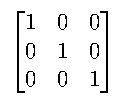
\includegraphics{identity_matrix}
  \caption{\gls*{identity-matrix}的示例:这是
    $\pmb{I}_3$\label{fig:identity_matrix}}
\end{figure}

$\pmb{A}$ 的\gls*{matrix-inversion}表示为 $\pmb{A}^{-1}$,它被定义为这样的矩阵:
\begin{equation}
  \pmb{A}^{-1}\pmb{A} = \pmb{I}_n
  \label{eq:matrix-inverse}
\end{equation}

现在我们可以通过以下步骤解方程~\ref{eq:system_of_linear_equations}:
\begin{gather}
  \pmb{A}\pmb{x} = \pmb{b}\\
  \pmb{A}^{-1}\pmb{A}\pmb{x} = \pmb{A}^{-1}\pmb{b}\\
  \pmb{I}_n\pmb{x} = \pmb{A}^{-1}\pmb{b}\\
  \pmb{x} = \pmb{A}^{-1}\pmb{b}
\end{gather}

当然,这依赖于可能找到 $\pmb{A}^{-1}$。我们在接下来一节中讨论 $\pmb{A}^{-1}$ 存在
的条件。

当 $\pmb{A}^{-1}$ 存在时,存在几种不同算法用于在闭合式中找到它。理论上,同样的逆
矩阵可以被用于多次解不同 $\pmb{b}$ 值的方程。然而,$\pmb{A}^{-1}$ 主要作为一个假
设的工具使用,实际上不应该被用在大多数软件应用中。由于在一个数字计算机
中 $\pmb{A}^{-1}$ 可以仅由有限精度表示,利用 $\pmb{b}$ 值的算法通常可以取得更精确
的 $\pmb{x}$ 的估算。

\section{线性相关和生成空间}
\label{sec:linear_dependence_and_span}

为使 $\pmb{A}^{-1}$ 存在,方程~\ref{eq:system_of_linear_equations} 必须对每
个 $\pmb{b}$ 的值有唯一的解。然而,方程系对有些 $\pmb{b}$ 的值也可能无解或有无限
多解。对一个特定的 $\pmb{b}$ 不可能有介于一个和无限多个之间的解;如果 $\pmb{x}$
和 $\pmb{y}$ 都是解,那么
\begin{equation}
  \pmb{z} = \alpha\pmb{x} + (1 - \alpha)\pmb{y}
\end{equation}
对于任意实数 $\alpha$ 也是一个解。

为了分析方程有多少解,我们可以把 $\pmb{A}$ 的列看做指向从\textbf{原点}(由全部
为 $0$ 的向量指定的点)出发的不同方向,并确定有多少路径到达 $\pmb{b}$。在这个观点
下,$\pmb{x}$ 的每个元素指定了我们沿着每个方向要走多远,这里 $x_i$ 指定沿着
列 $i$ 移动多远:
\begin{equation}
  \pmb{A}\pmb{x} = \sum_{i}x_i\pmb{A}_{:,i}
\end{equation}

通常,这种类型的操作被称为\emph{\gls{linear-comb}}。正式地,一个由一
组\gls*{vecs} ${\pmb{v}^{(1)}, \ldots, \pmb{v}^{(i)}}$ 构成的\gls*{linear-comb},
是将每个\gls*{vec} $\pmb{v}^{(i)}$ 乘以一个相应的标量系数并且把结果相加:
\begin{equation}
  \sum_{i}c_i\pmb{v}^{(i)}
\end{equation}

一组向量的\emph{\gls{span}}\,是由原始\gls*{vecs}的\gls*{linear-comb}得到的所有点
的集合。

确定 $\pmb{A}\pmb{x} = \pmb{b}$ 是否有一个解,相当于测试 $\pmb{b}$ 是否
在 $\pmb{A}$ 列中的\gls*{span}。这个特定的\gls*{span}被称
为\emph{\gls{column-space}}\,或者 $\pmb{A}$ 的\emph{\gls{range}}。

为了使方程系 $\pmb{A}\pmb{x} = \pmb{b}$ 对所有 $\pmb{b} \in \mathbb{R}^m$ 的所有
值有唯一解,我们需要 $\pmb{A}$ 的所有\gls*{column-space}为 $\mathbb{R}$。如
果 $\mathbb{R}^m$ 中的任何点被排除于\gls*{column-space}之外,那个点是一个潜在的无
解的 $\pmb{b}$ 值。$\pmb{A}$ 的所有\gls*{column-space}是 $\mathbb{R}^m$ 的需求,
立即暗示了 $\pmb{A}$ 必须有至少 $m$ 个列,即 $n \geq m$。否
则,\gls*{column-space}的维度会小于 $m$。例如,考虑一个 $3 \times 2$ 的矩阵。目
标 $\pmb{b}$ 是 3 维的,但是 $\pmb{x}$ 仅仅是 2 维,所以修改 $\pmb{x}$ 的值最好情
况下允许我们描绘出一个 $\mathbb{R}^3$ 中的 2 维平面。方程当且仅当 $\pmb{b}$ 位于
平面上时有一个解。

对于每个点有一个解,$n \geq m$ 仅仅是一个必要条件。它不是充分条件,因为有可能一些
列是冗余的。考虑一个 $2 \times 2$ 的矩阵,其中两列都是相同的。这与一个仅含有一个
重复列的 $2 \times 1$ 的矩阵 有相同的\gls*{column-space}。换句话说,即使有两
列,\gls*{column-space}仍然仅仅是一条线,无法包含所有的 $\mathbb{R}^2$。

正式地,这种冗余被称为\emph{\gls{linear-dep}}。一个\gls*{vecs}集,如果其中没有一
个\gls*{vec}是其它集和中\gls*{vecs}的\gls*{linear-comb},那么这
个\gls*{vecs}集是\emph{\gls{linearly-indep}}\,的。如果我们往集合中加上一
个\gls*{vec},它是一个集合中其它\gls*{vecs}的\gls*{linear-comb},那么新
的\gls*{vec}并不往集合的\gls*{span}中增加任何点。这意味着对于矩阵
的\gls*{column-space}要包含所有 $\mathbb{R}^m$,这个矩阵必须含有至少一
个 $m$ 个\gls*{linearly-indep}列的集合。这个条件是方
程~\ref{eq:system_of_linear_equations} 的必要条件和充分条件,使得方程对每
个 $\pmb{b}$ 值有一个解。注意这个需求中的集合,是正好
有 $m$ 个\gls*{linear-indep}的列,不是至少 $m$ 列。没有 $m$ 维\gls*{vecs}的集合可
以有多于 $m$ 个互相\gls*{linearly-indep}的列,但是一个具有多于 $m$ 列的矩阵可能有
多于一个这样的集合。

为了使矩阵有一个转置,我们另外需要确保方程~\ref{eq:system_of_linear_equations} 对
每一个 $\pmb{b}$ 的值\textbf{最多}有一个解。为此,我们需要确保矩阵有最多 $m$ 个列。
否则就有多于一个方法来确定每个解的参数。

综合起来,这意味着矩阵必须是\emph{\gls{square}},即,我们需要 $m = n$ 并且所有的
列必须是\gls*{linearly-indep}。一个具有\gls*{linearly-dep}列的方块矩阵被称
为\emph{\gls{singular}}。

如果 $\pmb{A}$ 不是矩阵或者是方块矩阵但不是\gls*{singular},仍然可能解这个方程。
但是我们不能使用\gls*{matrix-inversion}的方法来找出解。

目前为止我们已经讨论过了在左边乘的逆矩阵。也可能定义一个在右边乘的逆:
\begin{equation}
  \pmb{A}\pmb{A}^{-1} = \pmb{I}
\end{equation}

对于方块矩阵,左边求逆和右边求逆是相同的。

\section{范数}
\label{sec:norms}

有时候我们需要测量一个\gls*{vec}的长度。在\gls*{ml}中,我们通常使用一个被称
为\emph{\gls{norm}}\,的函数测量\gls*{vecs}的长度。正式地,对于
$p \in \mathbb{R}, p \geq 1$,$L^p$ 的范数由
\begin{equation}
  \|\pmb{x}\|_p = \left(\sum_i|x_i|^p\right)^{\frac{1}{p}}
  \label{eq:lp_norm}
\end{equation}
给出。

这些范数,包括 $L^p$ 范数,是将\gls*{vecs}映射为非负值的函数。凭直觉地,一
个\gls*{vec} $\pmb{x}$ 的范数测量从原点到点 $\pmb{x}$ 的距离。更严格地,一个范数
是满足以下特性的任意函数 $f$:
\begin{itemize}
\item $f(\pmb{x}) = 0 \Rightarrow \pmb{x} = \pmb{0}$
\item $f(\pmb{x} + \pmb{y}) \leq f(\pmb{x}) + f(\pmb{y})$
  (\emph{\gls{tri-inequal}}\,)
\item $\forall \alpha \in \mathbb{R}, f(\alpha \pmb{x}) = |\alpha|f(\pmb{x})$
\end{itemize}

具有 $p = 2$ 的 $L^2$ 范数被称为\emph{\gls{eu-norm}}。它是从原点到点 $\pmb{x}$ 的
欧几里德距离。$L^2$ 范数被频繁地使用在\gls*{ml}中以至于它常常被简单表示
为 $\|\pmb{x}\|$,而忽略其下标 $2$。通常也使用平方 $L^2$ 范数测量一个\gls*{vec}的
长度,它可以简单地由 $\pmb{x}^{\top}\pmb{x}$ 来计算。

平方 $L^2$ 范数在数学和计算上比 $L^2$ 范数本身更方便。例如,每个平方 $L^2$ 范数对
于每一个 $\pmb{x}$ 元素的导数,仅依赖于对应的 $\pmb{x}$ 的元素,而所有 $L^2$ 范数
的导数依赖于整个\gls*{vec}。在许多环境中,平方 $L^2$ 范数可能是不受欢迎的,因为它
在原点附近缓慢地增长。在几个\gls*{ml}应用中,区分完全为 $0$ 的元素和很小但非 $0$
的元素是很重要的。在这些情况下,我们转而采用一个在所有位置以相同速率增长,但是在
数学上保留简单特性的函数:$L^1$ 范数。$L^1$ 范数可以简化为:
 \begin{equation}
  \|\pmb{x}\|_1 = \sum_i|x_i|
\end{equation}

当 $0$ 和 非 $0$ 元素非常重要时,$L^1$ 范数被普遍使用在\gls*{ml}中。每次一
个 $\pmb{x}$ 元素从 $0$ 移动了 $\epsilon$,$L^1$ 范数增加了 $\epsilon$。

我们有时候通过计算非 $0$ 元素的个数来测量\gls*{vec}的大小。有些作者把这个函数表示
为``$L^0$''范数,但这是个错误的术语。一个\gls*{vec}中的非 $0$ 元素的个数不是一个
范数,因为通过 $\alpha$ 来调整\gls*{vec}不改变非 $0$ 元素的个数。$L^1$ 模常常被用
作非 $0$ 元素个数的代替者。

另一个在\gls*{ml}中普遍出现的范数是
$L^{\infty}$,也被称为\emph{\gls{max-norm}}。这个范数简化为\gls*{vec}中最大幅度元
素的绝对值,
\begin{equation}
  \|\pmb{x}\|_{\infty} = \max_i|x_i|
\end{equation}

有时候我们也想要测量矩阵的大小。在\gls*{dl}的环境中,最普遍的方式是以不同的、费解
的\emph{\gls{fr-norm}}
\begin{equation}
  \|A\|_F = \sqrt{\sum_{i,j}A_{i,j}^2}
\end{equation}
它类似于一个\gls*{vec}的 $L^2$ 范数。

两个\gls*{vecs}的点乘可以重写为范数的形式。具体来说,
\begin{equation}
  \pmb{x}^{\top}\pmb{y} = \|\pmb{x}\|_2\|\pmb{y}\|_2\cos \theta
\end{equation}
其中 $\theta$ 是 $\pmb{x}$ 和 $\pmb{y}$ 之间的夹角。

\section{特殊类型的矩阵和向量}
\label{sec:special_kinds_of_matrices_and_vectors}

一些特别有用的特殊类型的矩阵和\gls*{vecs}。

\emph{\gls{diag}}\,矩阵大部分由 $0$ 组成,仅仅沿着主对角线有非 $0$ 元素。正式地,
一个矩阵 $\pmb{D}$ 当且仅当对所有 $i \neq j$ 的 $D_{i,j} = 0$ 时是对角线的。我们
已经见过了一个对角矩阵的例子:单位矩阵,其中所有的对角线元素为 $1$。我们写
成 $\mathrm{diag}(\pmb{v})$ 来表示一个方块对角矩阵,其中对角线元素由\gls*{vec}
$\pmb{v}$ 的元素给出。对角矩阵在某种程度上让人感兴趣是因为被一个对角矩阵相乘,在
计算上是非常有效率的。计算 $\mathrm{diag}(\pmb{v})\,\pmb{x}$,我们只需要用 $v_i$
来调整每个元素
$x_i$。换句话说,$\mathrm{diag}(\pmb{v})\,\pmb{x} = \pmb{v} \odot \pmb{x}$。对一
个方块对角矩阵求逆也同样高效。仅当每个对角线元素为非 $0$ 时矩阵的逆存在,在这种情
况下,$\mathrm{diag}(\pmb{v})^{-1} = \mathrm{diag}([1/v_1, \ldots,
1/v_n]^{\top})$。在许多情况下,我们可能会得到一些非常一般的以任意矩阵形式
的\gls*{ml}算法,但通过限制一些矩阵为对角矩阵可获得一个代价更低的(和更少描述性的)
算法。

不是所有的对角矩阵需要是方块型的。构建一个矩形的对角矩阵是可能的。非方块对角矩阵
没有逆,但是它仍然可能被它们以较低的代价相乘。对于一个非方块对角矩阵 $\pmb{D}$,
乘积 $\pmb{D}\pmb{x}$ 会涉及到调整 $\pmb{x}$ 的每个元素,并且,如果 $\pmb{D}$ 的
高度比宽度大则往结果中连接一些 $0$,或者当 $\pmb{D}$ 的宽度大于高度时则舍
弃\gls*{vec}的最后一些元素。

一个\emph{\gls{symmetric}}\,矩阵是任何和其自身的转置相等的矩阵:
\begin{equation}
  \pmb{A} = \pmb{A}^{\top}
\end{equation}
对称矩阵常常出现在其中的元素由一些有两个参数的函数生成的时候,其元素不依赖于这两
个参数的顺序。例如,如果 $\pmb{A}$ 是一个距离测量的矩阵,$\pmb{A}_{i,j}$ 给出了从
点 $i$ 到点 $j$ 的距离,那么因为距离函数是对称的,$\pmb{A}_{i,j} =
\pmb{A}_{j,i}$。

一个\emph{\gls{unit-vec}}\,是一个具有\emph{\gls{unit-norm}}\,的\gls*{vec}:
\begin{equation}
  \|\pmb{x}\|_2 = 1
\end{equation}

一个\gls*{vec} $\pmb{x}$ 和一个 \gls*{vec} $\pmb{y}$,如
果 $\pmb{x}^{\top}\pmb{y} = 0$,那么它们是相互\emph{\gls{ortho}}。如果两
个\gls*{vecs}都有非 $0$ \gls*{norm},这意味着它们以 $90^{\circ}$ 角相互垂直。
在 $\mathbb{R}^n$ 中,最多有 $n$ 个具有非 $0$ \gls*{norm}的\gls*{vecs}可以相互正
交。如果\gls*{vecs}不仅是正交的,还有\gls*{unit-norm},那么我们称它们
是\emph{\gls{orthonormal}}。

一个\emph{\gls{orthonormal-matrix}}\,是一个方块矩阵,其各行是相
互\gls*{orthonormal},而各列也是相互\gls*{orthonormal}:
\begin{equation}
  \pmb{A}^{\top}\pmb{A} = \pmb{A}\pmb{A}^{\top} = \pmb{I}
\end{equation}

这表示
\begin{equation}
  \pmb{A}^{-1} = \pmb{A}^{\top}
\end{equation}
所以正交矩阵有趣在它们的逆可以以很低的代价来计算。认真注意正交矩阵的定义。相反,
它们的行不仅仅是正交的,而且是完全标准正交的。没有一个特殊的术语来定义一个行或列
正交但不是标准正交的矩阵。

\section{特征分解}
\label{sec:eigendecomposition}

通过把整体分解成多个组成部分,或者找到一些具有普遍性的特性而不是我们选择来表示的
方式,许多数学对象能够被更好理解。

例如,整数能够被分解成素数因子。我们表示数字 $12$ 的方式会随着我们以十进制或者二
进制的方式而改变,但总会是 $12 = 2 \times 2 \times 3$。从这样的表示我们可以最终得
到有用的特性,诸如 $12$ 不能被 $5$ 除,或者任意乘以 $12$ 后能被 $3$ 除。

正如我们通过把一个整数分解为素数因子来发现某些整数的真实性质,我们也能以显示关于
矩阵的功能特性的方式~——~这些特性从一个元素数组的表示中并不明显~——~分解它们。

一个最广泛使用的矩阵分解被称为\emph{\gls{eigen-decompos}},使用它我们把一个矩阵分
解为一系列特征向量和特征值的集合。

一个方块矩阵 $\pmb{A}$ 的\emph{\gls{eigen-vec}}\,是这样一个非 $0$ 向量 $\pmb{v}$,
它被 $\pmb{A}$ 乘后仅仅改变了 $\pmb{v}$ 的缩放:
\begin{equation}
  \pmb{A}\pmb{v} = \lambda\pmb{v}
\end{equation}
缩放因子 $\lambda$ 被称为相对于这个\gls*{eigen-vec}的\emph{\gls{eigen-val}}。(也
可以找到一个\emph{\gls{left-eigen-vec}},这样
$\pmb{v}^{\top}\pmb{A} = \lambda\pmb{v}^{\top}$,但是我们通常关注的是
右\gls*{eigen-vec})。

如果 $\pmb{v}$ 是 $\pmb{A}$ 的一个\gls*{eigen-vec},那么对于 $s \in \mathbb{R},
s \neq 0$ 的任意缩放的\gls*{vec} $s\pmb{v}$,$s\pmb{v}$ 也是如此。此
外,$s\pmb{v}$ 仍然有相同的\gls*{eigen-val}。因为这个原因,我们通常只找单
位\gls*{eigen-vecs}。

假设矩阵 $\pmb{A}$ 有
$n$个线性不相关的\gls*{eigen-vecs},$\{\pmb{v}^{(1)}, \ldots, \pmb{v}^{(n)}\}$,
并有相应的\gls*{eigen-vals}
$\{\lambda_1, \ldots, \lambda_n\}$。我们可以把所有\gls*{eigen-vecs}串联起来形成一
个每列有一个\gls*{eigen-vec}的矩阵$\pmb{V}$:$\pmb{V} = [\pmb{v}^{(1)}, \ldots,
\pmb{v}^{(n)}]$。同样地,我们能够把\gls*{eigen-vals}串联起来形成一个\gls*{vec}
$\pmb{\lambda} = [\lambda_1, \ldots, \lambda_n]^{\top}$。那么 $\pmb{A}$ 的特征分
解就由
\begin{equation}
  \pmb{A} = \pmb{V}\mathrm{diag}(\pmb{\lambda})\pmb{V}^{-1}
\end{equation}
给出。

我们已经看到\textbf{构建}具有特定的\gls*{eigen-vals}和\gls*{eigen-vecs}的矩阵允许
我们在期望的方向上伸展空间。然而,我们往往想要把矩阵\textbf{分解}为他们
的\gls*{eigen-vals}和\gls*{eigen-vecs}。这样做可以帮助我们分析矩阵的某些属性,就
像把一个整数分解成它的素数因子,可以帮助我们了解该整数的行为。

不是每个矩阵能够被分解为\gls*{eigen-vals}和\gls*{eigen-vecs}。在某些情况下,存在
这样的分解,但可能涉及到复数而不是实数。幸运地,在这本书中,我们通常只需要分解一
些特殊的、有着简单分解的矩阵类别。特别地,只使用实数值
的\gls*{eigen-vecs}和\gls*{eigen-vals},每一个实数对称矩阵能够被分解为一个表达
式:
\begin{equation}
  \pmb{A} = \pmb{Q}\pmb{\Lambda}\pmb{Q}^{\top}
\end{equation}
其中 $\pmb{Q}$ 是一个由\gls*{eigen-vecs} $\pmb{A}$ 组成的正交矩阵,
而 $\pmb{\Lambda}$ 是一个对角矩阵。\gls*{eigen-val} $\Lambda_{i,i}$ 与 $\pmb{Q}$
的第 $i$ 列~——~表示为 $\pmb{Q}_{:,i}$~——~中的\gls*{eigen-vec}相关。由
于 $\pmb{Q}$ 是一个正交矩阵,我们可以把 $\pmb{A}$ 看做通过 $\pmb{v}^{(i)}$ 方向上
的 $\lambda_i$ 调整的缩放空间。参见
图~\ref{fig:effect_of_eigenvectors_and_eigenvalues} 的示例。

\begin{figure}[h]
  \centering
  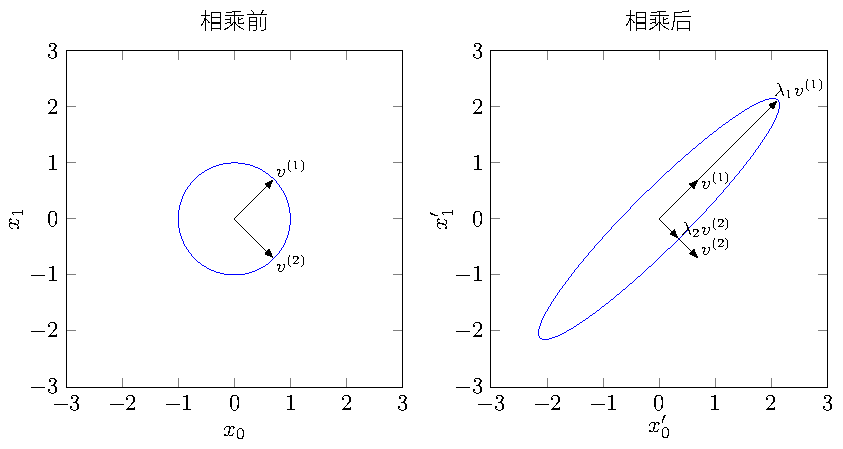
\includegraphics{eigen_effect}
  \caption{一个\gls*{eigen-vecs}和\gls*{eigen-vals}影响的示例。这里我们有一个矩
    阵 $\pmb{A}$,它有两
    个\gls*{orthonormal}\gls*{eigen-vecs},有\gls*{eigen-val}
    $\lambda_1$ 的 $\pmb{v}^{(1)}$ 和有\gls*{eigen-val}
    $\lambda_2$ 的 $\pmb{v}^{(2)}$。(\textbf{左边})我们把所有单位\gls*{vecs}
    $\pmb{u} \in \mathbb{R}^2$ 的集合绘成一个单位圆。(\textbf{右边})我们绘上了
    所有点 $\pmb{A}\pmb{u}$ 的集合。通过观察 $\pmb{A}$ 扭曲单位圆的方式,我们能够
    看到它在 $\pmb{v}^{(i)}$ 方向上被 $\lambda_i$ 缩放了空间。
    \label{fig:effect_of_eigenvectors_and_eigenvalues}}
\end{figure}

虽然任何实数对称矩阵 $\pmb{A}$ 可确保有一个特征分解,但它可能不是唯一的。如果有两
个或两个以上的\gls*{eigen-vecs}共享相同的\gls*{eigen-val},那么任何一组位于它们生
成空间的正交\gls*{vecs}也是具有那个\gls*{eigen-val}的\gls*{eigen-vecs},而我们可
以等价地用这些\gls*{eigen-vecs}选择一个 $\pmb{Q}$。按照惯例,我们通常以降序排
序 $\Lambda$ 中的元素。在这种惯例下,只有当所有的\gls*{eigen-vals}是唯一时,特征
分解是唯一的。

矩阵的特征分解告诉我们很多关于矩阵的有用的事实。当且仅当任
何\gls*{eigen-vals}是 $0$ 时,矩阵是奇异的。一个实数对称矩阵的特征分解也能够被用
于以 $\|\pmb{x}\|_2 = 1$ 的条件优化 $f (\pmb{x}) = \pmb{x}^{\top}$ 形式的二次方表
达式。当 $\pmb{x}$ 等于一个 $\pmb{A}$ 的\gls*{eigen-vec}时,$f$ 的取值是相应
的\gls*{eigen-val}。$f$ 在约束域内的的最大值是\gls*{eigen-val}的最大值,它在约束
域内的最小值是\gls*{eigen-val}的最小值。

一个\gls*{eigen-vals}都是正数的矩阵被称为\emph{\gls{positive-definite}}。一
个\gls*{eigen-vals}都是正数或者 $0$ 的矩阵被称
为\emph{\gls{positive-semidefinite}}。相同地,如果所有的\gls*{eigen-vals}都是负数,
那么矩阵是\emph{\gls{negative-definite}},而如果所有\gls*{eigen-vals}都是负数或
者 $0$,它是\emph{\gls{negative-semidefinite}}。\gls*{positive-semidefinite}有趣
在它们确保
$\forall\pmb{x}, \pmb{x}^{\top}\pmb{A}\pmb{x} \geq 0$。\gls*{positive-definite}另
外能确保 $\pmb{x}^{\top}\pmb{A}\pmb{x} = 0 \Rightarrow \pmb{x} = 0$.

\section{奇异值分解}
\label{sec:singular_value_decomposition}

在~\ref{sec:eigendecomposition} 一节,我们看到了如何将一个矩阵分解
为\gls*{eigen-vecs}和\gls*{eigen-vals}。\emph{\gls{svd}}(SVD)提供了另一种分解一
个矩阵为\emph{\gls{singular-vecs}}\,和\emph{\gls{singular-vals}}\,的方式。SVD允许
我们去发现一些和特征分解相同类型的信息。然而,SVD 更普遍适用。每一个实数矩阵有一
个\gls*{singular-val}分解,但\gls*{eigen-val}分解不是。例如,如果一个矩阵不是方块
的,那么就没有特征分解,相反我们必须使用一个\gls*{singular-val}分解。

回忆一下特征分解涉及到分析一个矩阵 $\pmb{A}$ 来发现一个\gls*{eigen-vecs}的矩
阵 $\pmb{V}$ 和一个\gls*{eigen-vals}的\gls*{vec} $\pmb{\lambda}$,这样我们可以重
写$\pmb{A}$ 为:
\begin{equation}
  \pmb{A} = \pmb{V}\mathrm{diag}(\pmb{\lambda})\pmb{V}^{-1}
\end{equation}

\gls*{singular-val}分解类似,只是这次我们把 $\pmb{A}$ 写为三个矩阵的乘积:
\begin{equation}
  \pmb{A} = \pmb{U}\pmb{D}\pmb{V}^{\top}
\end{equation}

假设 $\pmb{A}$ 是一个 $m \times n$ 的矩阵。那么 $\pmb{U}$ 被定义为一个 $m \times
n$ 的矩阵,$\pmb{D}$ 是一个 $m \times n$ 的矩阵,$\pmb{V}$ 是一个 $n \times n$的
矩阵。

这些矩阵每个都被定义为具有一个特殊结构。矩阵 $\pmb{U}$ 和 $\pmb{V}$ 都被定义为正
交矩阵。矩阵 $\pmb{D}$ 被定义为一个对角矩阵。注意 $\pmb{D}$ 不是必须为方块矩阵。

沿着 $\pmb{D}$ 对角线的元素被称为矩
阵 $\pmb{A}$ 的\emph{\gls{singular-val}}。$\pmb{U}$ 的列被称
为\emph{\gls{left-singular-vecs}}。$\pmb{V}$ 的列被称
为\emph{\gls{right-singular-vecs}}。

实际上我们可以以 $\pmb{A}$ 的特征分解的功能方面来解
释 $\pmb{A}$ 的\gls*{singular-val}分
解。$\pmb{A}$ 的\gls*{left-singular-vecs}是$\pmb{A}\pmb{A}^{\top}$ 的
\gls*{eigen-vecs}。$\pmb{A}$ 的\gls*{right-singular-vecs}是
$\pmb{A}^{\top}\pmb{A}$ 的\gls*{eigen-vecs}。$\pmb{A}$ 的非 $0$
\gls*{singular-vals}是 $\pmb{A}^{\top}\pmb{A}$ 的\gls*{eigen-vecs}的平方根。对
于 $\pmb{A}\pmb{A}^{\top}$ 也一样。

也许 SVD 最有用的功能,是我们能够用它来部分归纳出非方块矩阵的逆矩阵,正如我们在接
下来一节会看到的。

\section{摩尔--彭若斯广义逆}
\label{sec:the_moore_penrose_pseudoinverse}

矩阵求逆并不是为非方块的矩阵定义的。假设我们想要取得一个矩阵 $\pmb{A}$ 的左逆矩
阵 $\pmb{B}$,以便我们可以通过左乘每一边得到
\begin{equation}
  \pmb{x} = \pmb{B}\pmb{y}
\end{equation}
来解一个线性方程
\begin{equation}
  \pmb{A}\pmb{x} = \pmb{y}
\end{equation}

依赖于这个问题的结构,有可能不能设计一个唯一的从 $\pmb{A}$ 到 $\pmb{B}$ 的映射。

如果 $\pmb{A}$ 的高大于它的宽,那么这个方程有可能无解。如果 $\pmb{A}$ 的宽大于高,
那么有可能有多个解。

\emph{\gls{moore-penrose-pseudoinverse}}\,允许我们在这种情况下取得进
展。$\pmb{A}$ 的广义逆被定义为一个矩阵
\begin{equation}
  \pmb{A}^+ = \lim_{\alpha \searrow 0}(\pmb{A}^+\pmb{A} +
  \alpha\pmb{I})^{-1}\pmb{A}^{\top}
\end{equation}
实际为了计算这个广义逆的算法并不是基于这个定义,而是这个公式
\begin{equation}
  \pmb{A}^+ = \pmb{V}\pmb{D}^+\pmb{U}^{\top}
\end{equation}
其中 $\pmb{U}$,$\pmb{D}$ 和 $\pmb{V}$ 是 $\pmb{A}$ 的\gls*{singular-val}分解,而
一个对角矩阵 $\pmb{D}$ 的广义逆 $\pmb{D}^+$ 是通过取它的非 $0$ 元素的倒数然后取所
得矩阵的转置得到的。

当 $\pmb{A}$ 的列数多于行数,那么使用广义逆解一个线性方程提供了许多可能解中的一个。
明确地,它给出在所有可能的解中具有最小欧几里得范数 $\|\pmb{x}\|_2$ 的解$\pmb{x}
= \pmb{A}^+\pmb{y}$。

当 $\pmb{A}$ 的行数多于列数,可能无解。在这种情况下,使用广义逆为我们给出了就欧几
里得范数 $\|\pmb{A}\pmb{x} - \pmb{y}\|_2$ 而言使得 $\pmb{A}\pmb{x}$ 尽可能接
近$\pmb{y}$ 的 $\pmb{x}$ 值。

\section{迹算子}
\label{sec:the_trace_operator}

迹算子给出了一个矩阵的所有对角线元素的和:
\begin{equation}
  \mathrm{Tr}(\pmb{A}) = \sum_i\pmb{A}_{i,i}
\end{equation}

迹算子之所以有用是有多种原因的。一些不借助求和符号难于具体说明的算子,能够使用矩
阵乘积和迹算子来说明。例如,迹算子提供了一个写出矩阵的弗罗贝尼乌斯范数的替代方
法:
\begin{equation}
  \|A\|_F = \sqrt{\mathrm{Tr}(\pmb{A}\pmb{A}^{\top})}
  \label{eq:trace_operator_of_frobenius_norm}
\end{equation}

以迹算子的形式写一个表达式开辟了利用许多有用特性来处理表达式的机会。例如,迹算子
作用于转置算子后不变:
\begin{equation}
  \mathrm{Tr}(\pmb{A}) = \mathrm{Tr}(\pmb{A}^{\top})
\end{equation}

由许多因子组成的方块矩阵,如果相应矩阵的形状允许得到的乘积有定义,这个方块矩阵的
迹,对于将最后的因子移到首位也不变:
\begin{equation}
  \mathrm{Tr}(\pmb{A}\pmb{B}\pmb{C}) = \mathrm{Tr}(\pmb{C}\pmb{A}\pmb{B}) =
  \mathrm{Tr}(\pmb{B}\pmb{C}\pmb{A})
\end{equation}
或者更普遍地,
\begin{equation}
  \mathrm{Tr}(\prod^n_{i=1}\pmb{F}^{(i)} =
  \mathrm{Tr}(\pmb{F}^{(n)}\prod^{n-1}_{i=1}\pmb{F}^{(i)})
  \label{eq:trace_of_square_matrix}
\end{equation}
这个循环排列的不变性即使当得到的乘积有一个不同的形状仍然保持成立。例如,对
于 $\pmb{A} \in \mathbb{R}^{m \times n}$ 和
$\pmb{B} \in \mathbb{R}^{n \times m}$,即使
$\pmb{A}\pmb{B} \in \mathbb{R}^{m \times m}$ 和
$\pmb{B}\pmb{A} \in \mathbb{R}^{n \times n}$,我们有
\begin{equation}
  \mathrm{Tr}(\pmb{A}\pmb{B}) = \mathrm{Tr}(\pmb{B}\pmb{A})
\end{equation}

另一个要记住的有用的事实是一个标量是它自身的迹:$a = \mathrm{Tr}(a)$。

\section{行列式}
\label{sec:the_determinant}

一个方块矩阵的行列式,表示为
$\det(\pmb{A})$,是一个将矩阵映射为实数标量的函数。行列式等于矩阵的所
有\gls*{eigen-vals}的乘积。行列式的绝对值可以被看作是衡量被矩阵相乘后扩展或者压缩
了多少空间。如果行列式为 $0$,那么空间被完全沿着至少一个维度压缩,导致它丢失了所
有体积。如果行列式为 $1$,那么变换是保体积的。

\section{示例:主成分分析}
\label{sec:example:principal_components_analysis}

一个简单的\gls*{ml}算法,\emph{\gls{pca}}\,或者 \emph{PCA},能够仅仅利用线性代数
的基本知识来推导。

假设我们在 $\mathbb{R}^n$ 中有一个 $m$ 个点的集合
$\{\pmb{x}^{(1)}, \ldots, \pmb{x}^{(m)}\}$。假设我们想要在这些点上应用有损数据压
缩。有损数据压缩意味着以一个需要更少内存但是可能丢失一些精度的方式存储这些点。我
们想要丢失尽可能少的精度。

一种我们能对这些点进行编码的方式是表示它们的一个低维度版本。对每个
点 $\pmb{x}^{(i)} \in \mathbb{R}^n$,我们能找到一个相应的编码向量
$\pmb{c}^{(i)} \in \mathbb{R}^l$。如果 $l$ 小于 $n$,它会用比原始数据更少内存用于
存储编码的点。我们想要找到某个编码函数
$f(\pmb{x}) = \pmb{c}$,它为一个输入生成编码,以及一个解码函数,给定它的编码生成
重构的输入,$\pmb{x} \approx g(f(\pmb{x}))$。

PCA 是由我们选择的解码函数定义的。更明确地说,要使得解码非常简单,我们选择使用矩
阵操作来将编码映射回 $\mathbb{R}^n$。让 $g(\pmb{c}) = \pmb{D}\pmb{c}$,其
中 $\pmb{D} \in \mathbb{R}^{n \times l}$ 是定义解码的矩阵。

为这个解码器计算最优的编码可能是一个困难的问题。为了让编码问题保持简
单,PCA 将 $\pmb{D}$ 的列限制为彼此正交。(注意 $\pmb{D}$ 严格地说仍然不是``一个
正交矩阵'',除非 $l = n$)

随着目前所描述的问题,有可能有许多解,因为如果我们对所有点按比例减小 $c_i$ 我们能
够增加 $\pmb{D}_{:,i}$ 的规模。为了给出问题的唯一解,我们限制 $\pmb{D}$ 的所有列
具有单位\gls*{norm}。

为了将这个基本的思想转化为一个我们能够实现的算法,我们首先需要做的是计算出如何为
每个输入点 $\pmb{x}$ 产生最优的编码点 $\pmb{c}^*$。一种方法是最小化输入
点 $\pmb{x}$ 和它的复原值 $g(\pmb{c}^*)$ 之间的距离。我们可以用一个\gls*{norm}来
衡量这个距离。在主成分算法中,我们使用 $L^2$ \gls*{norm}:
\begin{equation}
  \pmb{c}^* = \mathop{\arg\min}_{\pmb{c}}\|\pmb{x} - g(\pmb{c})\|_2
\end{equation}

我们可以换成平方 $L^2$ \gls*{norm}而不是 $L^2$ \gls*{norm}自身,因为它们都被相同
的 $\pmb{c}$ 值最小化。这是因为 $L^2$ \gls*{norm}是非负的,而平方算子对非负参数是
单调增加的。
\begin{equation}
  \pmb{c}^* = \mathop{\arg\min}_{\pmb{c}}\|\pmb{x} - g(\pmb{c})\|^2_2
\end{equation}
被最小化的函数简化为
\begin{equation}
  (\pmb{x} - g(\pmb{c}))^{\top}(\pmb{x} - g(\pmb{c}))
\end{equation}
(由于 $L^2$ \gls*{norm}的定义,方程~\ref{eq:lp_norm})
\begin{equation}
  = \pmb{x}^{\top}\pmb{x} - \pmb{x}^{\top}g(\pmb{c}) - g(\pmb{c})^{\top}\pmb{x}
  + g(\pmb{c})^{\top}g(\pmb{c})
\end{equation}
(由于分配律)
\begin{equation}
  = \pmb{x}^{\top}\pmb{x} - 2\pmb{x}^{\top}g(\pmb{c}) +
  g(\pmb{c})^{\top}g(\pmb{c})
\end{equation}
(因为标量 $g(\pmb{x})^{\top}$ 等于其自身的转置)。

现在我们能再次改变正在被最小化的函数,来忽略第一项,因为这一项不依赖
于 $\pmb{c}$:
\begin{equation}
  \pmb{c}^* = \mathop{\arg\min}_{\pmb{c}} - 2\pmb{x}^{\top}g(\pmb{c}) +
    g(\pmb{c})^{\top}g(\pmb{c})
\end{equation}

为了更进一步,我们必须代入 $g(\pmb{c})$ 的定义:
\begin{gather}
  \pmb{c}^* = \mathop{\arg\min}_{\pmb{c}}-2\pmb{x}^{\top}\pmb{D}\pmb{c} +
  \pmb{c}^{\top}\pmb{D}^{\top}\pmb{D}\pmb{c}\\
  = \mathop{\arg\min}_{\pmb{c}}-2\pmb{x}^{\top}\pmb{D}\pmb{c} +
  \pmb{c}^{\top}\pmb{I}_l\pmb{c}
\end{gather}

(由于约束在 $\pmb{D}$ 上的正交性和单位\gls*{norm})
\begin{equation}
  = \mathop{\arg\min}_{\pmb{c}}-2\pmb{x}^{\top}\pmb{D}\pmb{c} +
  \pmb{c}^{\top}\pmb{c}
\end{equation}

我们能够使用\gls*{vec}微积分解这个最优化问题(如果你不知道怎么做,参
见~\ref{sec:gradient-based_optimization} 节):
\begin{gather}
  \nabla_{\pmb{c}}(-2\pmb{x}^{\top}\pmb{D}\pmb{c} + \pmb{c}^{\top}\pmb{c}) = 0\\
  -2\pmb{D}^{\top}\pmb{x} + 2\pmb{c} = 0\\
  \pmb{c} = \pmb{D}^{\top}\pmb{x}
\end{gather}

这使得算法更有效率:我们能够仅仅使用一个矩阵--\gls*{vec}算子来最优化地编
码 $\pmb{x}$。要编码一个\gls*{vec},我们应用编码器函数
\begin{equation}
  f(\pmb{x}) = \pmb{D}^{\top}\pmb{x}
\end{equation}
利用更进一步的矩阵操作,我们也能够定义 PCA 的重构算子:
\begin{equation}
  r(\pmb{x}) = g(f(\pmb{x})) = \pmb{D}\pmb{D}^{\top}\pmb{x}
  \label{eq:pca_reconstruction_operation}
\end{equation}

接下来,我们需要选择编码矩阵 $\pmb{D}$。为此,我们回顾下最小化输入和重构的 $L^2$
距离的想法。然而,既然我们会使用相同的矩阵 $\pmb{D}$ 来解码所有点,我们不能再孤立
地考虑这些点。相反,我们必须最小化在所有维度和所有点上计算的误差矩阵的弗罗贝尼乌
斯\gls*{norm}:
\begin{equation}
  \pmb{D}^* = \mathop{\arg\min}_{\pmb{D}}\sqrt{\sum_{i,j}(x^{(i)}_j -
    r(\pmb{x}^{(i)})_j)^2}\quad\text{使}\;\pmb{D}^{\top}\pmb{D} =
  \pmb{I}_l\;\text{满足}
  \label{eq:frobenius_norm_of_errors_matrix}
\end{equation}

为了推导找出 $\pmb{D}^*$ 的算法,我们开始会考虑 $l = 1$ 的情况。在这种情况
下,$\pmb{D}$ 仅仅是单个\gls*{vec},$\pmb{d}$。将方
程~\ref{eq:pca_reconstruction_operation} 代入方
程~\ref{eq:frobenius_norm_of_errors_matrix} 并将 $\pmb{D}$ 简化为 $\pmb{d}$,这个
问题缩小为
\begin{equation}
  \pmb{d}^* = \mathop{\arg\min}_{\pmb{d}}\sum_i\|\pmb{x}^{(i)} -
  \pmb{d}\pmb{d}^{\top}\pmb{x}^{(i)}\|^2_2\quad\text{使}\;\|\pmb{d}\|_2 =
  1\;\text{满足}
\end{equation}

上面的公式化是实施代入的最直接的方法,但在写方程的风格上不是最令人满意的方法。它
把标量值 $\pmb{d}^{\top}\pmb{x}^{(i)}$ 放在\gls*{vec} $\pmb{d}$ 的右边。把标量系
数写在它们作用于的\gls*{vec}更符合习惯。所以我们通常把这样一个公式写为
\begin{equation}
  \pmb{d}^* = \mathop{\arg\min}_{\pmb{d}}\sum_i\|\pmb{x}^{(i)} -
  \pmb{d}^{\top}\pmb{x}^{(i)}\pmb{d}\|^2_2\quad\text{使}\;\|\pmb{d}\|_2 =
  1\;\text{满足}
\end{equation}
或者,利用一个标量是它自身的转置这一事实,写为
\begin{equation}
  \pmb{d}^* = \mathop{\arg\min}_{\pmb{d}}\sum_i\|\pmb{x}^{(i)} -
  \pmb{x}^{(i)\top}\pmb{d}\pmb{d}\|^2_2\quad\text{使}\;\|\pmb{d}\|_2 =
  1\;\text{满足}
\end{equation}
读者应该力求变得熟悉这样的妆点性的重新整理。

到这里,以一个设计好的样本矩阵的形式,而不是在单独样本\gls*{vecs}上的求和,来重写
这个问题会更有帮助。这会允许我们使用更紧凑的符号。让 $\pmb{X} \in \mathbb{R}^{m
  \times n}$ 作为由整齐堆积所有描述这些点的\gls*{vecs}~——~诸如
$\pmb{X}_{i,:} = {x^{(i)}}^{\top}$~——~定义的矩阵。我们现在能够重写问题为
\begin{equation}
  \pmb{d}^* = \mathop{\arg\min}_{\pmb{d}}\sum_i\|\pmb{X} -
  \pmb{X}\pmb{d}\pmb{d}^{\top}\|^2_F\quad\text{使}\;\pmb{d}^{\top}\pmb{d} =
  1\;\text{满足}
\end{equation}

暂时忽略约束,我们能够如下简化弗罗贝尼乌斯范数部分:
\begin{gather}
  \mathop{\arg\min}_{\pmb{d}}\|\pmb{X} - \pmb{X}\pmb{d}\pmb{d}^{\top}\|^2_F\\ =
  \mathop{\arg\min}_{\pmb{d}}\mathrm{Tr}\,\bigg(\Big(\pmb{X} -
  \pmb{X}\pmb{d}\pmb{d}^{\top}\Big)^{\top}\Big(\pmb{X} -
  \pmb{X}\pmb{d}\pmb{d}^{\top}\Big)\bigg)
\end{gather}

(由于方程~\ref{eq:trace_operator_of_frobenius_norm})
\begin{gather}
  = \mathop{\arg\min}_{\pmb{d}}\mathrm{Tr}(\pmb{X}^{\top}\pmb{X} -
  \pmb{X}^{\top}\pmb{X}\pmb{d}\pmb{d}^{\top} -
  \pmb{d}\pmb{d}^{\top}\pmb{X}^{\top}\pmb{X} +
  \pmb{d}\pmb{d}^{\top}\pmb{X}^{\top}\pmb{X}\pmb{d}\pmb{d}^{\top})\\ =
  \mathop{\arg\min}_{\pmb{d}}\mathrm{Tr}(\pmb{X}^{\top}\pmb{X}) -
  \mathrm{Tr}(\pmb{X}^{\top}\pmb{X}\pmb{d}\pmb{d}^{\top}) -
  \mathrm{Tr}(\pmb{d}\pmb{d}^{\top}\pmb{X}^{\top}\pmb{X}) +
  \mathrm{Tr}(\pmb{d}\pmb{d}^{\top}\pmb{X}^{\top}\pmb{X}\pmb{d}\pmb{d}^{\top})\\ =
  \mathop{\arg\min}_{\pmb{d}} -
  \mathrm{Tr}(\pmb{X}^{\top}\pmb{X}\pmb{d}\pmb{d}^{\top}) -
  \mathrm{Tr}(\pmb{d}\pmb{d}^{\top}\pmb{X}^{\top}\pmb{X}) +
  \mathrm{Tr}(\pmb{d}\pmb{d}^{\top}\pmb{X}^{\top}\pmb{X}\pmb{d}\pmb{d}^{\top})
\end{gather}

(因为不涉及 $\pmb{d}$ 的项不影响 $\arg\min$)
\begin{equation}
  = \mathop{\arg\min}_{\pmb{d}} -
  2\mathrm{Tr}(\pmb{X}^{\top}\pmb{X}\pmb{d}\pmb{d}^{\top}) +
  \mathrm{Tr}(\pmb{d}\pmb{d}^{\top}\pmb{X}^{\top}\pmb{X}\pmb{d}\pmb{d}^{\top})
\end{equation}

(因为我们能够循环更替一个迹中矩阵的顺序,方程~\ref{eq:trace_of_square_matrix})
\begin{equation}
  = \mathop{\arg\min}_{\pmb{d}} -
  2\mathrm{Tr}(\pmb{X}^{\top}\pmb{X}\pmb{d}\pmb{d}^{\top}) +
  \mathrm{Tr}(\pmb{X}^{\top}\pmb{X}\pmb{d}\pmb{d}^{\top}\pmb{d}\pmb{d}^{\top})
\end{equation}

(再次使用相同的特性)

到这里,我们重新引入约束:
\begin{gather}
  \mathop{\arg\min}_{\pmb{d}} -
  2\mathrm{Tr}(\pmb{X}^{\top}\pmb{X}\pmb{d}\pmb{d}^{\top}) +
  \mathrm{Tr}(\pmb{X}^{\top}\pmb{X}\pmb{d}\pmb{d}^{\top}\pmb{d}\pmb{d}^{\top})
  \quad\text{使}\;\pmb{d}^{\top}\pmb{d} = 1\;\text{满足}\\
  = \mathop{\arg\min}_{\pmb{d}} -
  2\mathrm{Tr}(\pmb{X}^{\top}\pmb{X}\pmb{d}\pmb{d}^{\top}) +
  \mathrm{Tr}(\pmb{X}^{\top}\pmb{X}\pmb{d}\pmb{d}^{\top})
  \quad\text{使}\;\pmb{d}^{\top}\pmb{d} = 1\;\text{满足}
\end{gather}

(由于约束)
\begin{gather}
  = \mathop{\arg\min}_{\pmb{d}} -
  \mathrm{Tr}(\pmb{X}^{\top}\pmb{X}\pmb{d}\pmb{d}^{\top})
  \quad\text{使}\;\pmb{d}^{\top}\pmb{d} = 1\;\text{满足}\\
  = \mathop{\arg\min}_{\pmb{d}} 
  \mathrm{Tr}(\pmb{X}^{\top}\pmb{X}\pmb{d}\pmb{d}^{\top})
  \quad\text{使}\;\pmb{d}^{\top}\pmb{d} = 1\;\text{满足}\\
  = \mathop{\arg\min}_{\pmb{d}} 
  \mathrm{Tr}(\pmb{d}^{\top}\pmb{X}^{\top}\pmb{X}\pmb{d})
  \quad\text{使}\;\pmb{d}^{\top}\pmb{d} = 1\;\text{满足}
\end{gather}

这个最优化问题可以使用特征分解来解。明确地说,最优化的 $\pmb{d}$ 由对应于最大
的\gls*{eigen-val}的\gls*{eigen-vec} $\pmb{X}^{\top}\pmb{X}$ 给出。

在普遍情况下,$l > 1$,矩阵 $\pmb{D}$ 由对应于最大的\gls*{eigen-val}的 $l$
\gls*{eigen-vecs}给出。这可以使用归纳证明来显示。我们建议把写这个证明作为练习。

线性代数是理解\gls*{dl}所必需的基本数学学科之一。另一个\gls*{ml}中普遍存在的重要
的数学领域是概率论,接下来介绍。
